\begin{frame}
\frametitle{Khai báo vị trí viên đá}
Làm thế nào để người khác biết vị trí của viên đá đặc biệt đó?
\begin{figure}[H]
    \centering
    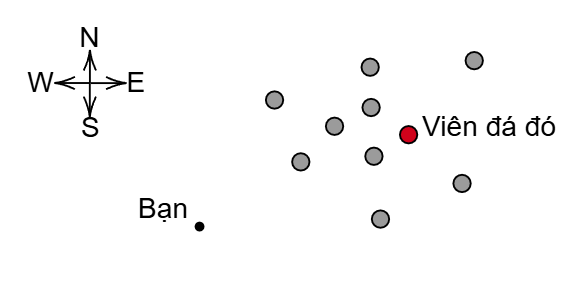
\includegraphics[width=10cm, height=5cm]{Slides/Figure/thestone.png}
\end{figure}
\end{frame}
\begin{frame}
    \frametitle{Cách 1}
    \begin{figure}[H]
        \centering
        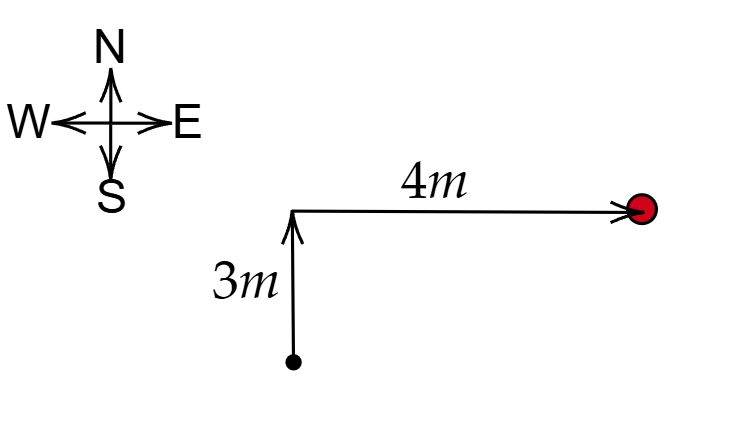
\includegraphics[width=8cm, height=5cm]{Slides/Figure/3m4m.png}
    \end{figure}
\end{frame}
\begin{frame}
    \frametitle{Cách 2}
    ``Chỉ tay'' và ``khoảng cách''
    \begin{figure}[H]
        \centering
        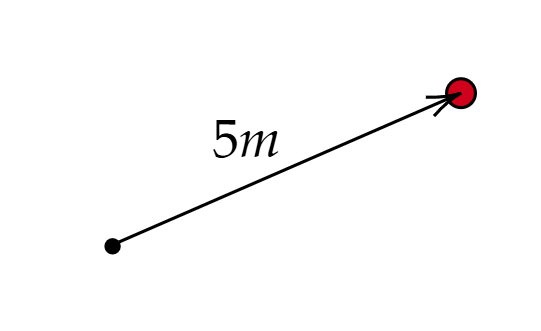
\includegraphics[width=8cm, height=5cm]{Slides/Figure/5m.png}
    \end{figure}
\end{frame}

\begin{frame}
\frametitle{Định nghĩa}
\begin{tcolorbox}[colback=blue!10, colframe=blue!50!black, title=Định nghĩa]
    Vector \(AB\) (hình vẽ), kí hiệu là \(\mathbf{AB}\), là một đại lượng biểu diễn bằng mũi tên tuân theo quy tắc hình bình hành được đặc trưng bởi độ dài \(a\) của nó (do đó còn được kí hiệu là \(\mathbf{a}\)) và hướng mà nó chỉ.
\end{tcolorbox}
    \begin{figure}[H]
    \centering
    
\includegraphics[width=1\textwidth]{Slides/Figure/vectorAB.png}
\end{figure}
\end{frame}